%!TEX program = xelatex
\documentclass[dvipsnames, svgnames,a4paper,11pt]{article}
% ----------------------------------------------------
%   吉林大学通信工程学院信号与系统实验报告
%   原作者:Huanyu Shi,2019级
%     知乎:https://www.zhihu.com/people/za-ran-zhu-fu-liu-xing
%     Github:https://github.com/huanyushi/SYSU-SPA-Labreport-Template
%   在原基础上魔改了一些,更加贴近吉林大学实验格式。
% ----------------------------------------------------

% ----------------------------------------------------- 
%	加边框的命令
%	参考:https://tex.stackexchange.com/questions/531559/how-to-add-the-page-border-for-first-two-pages-in-latex
\usepackage{tikz}
\usetikzlibrary{calc}
\usepackage{eso-pic}
\AddToShipoutPictureBG{%
\begin{tikzpicture}[overlay,remember picture]
\draw[line width=0.6pt] % 边框粗细
    ($ (current page.north west) + (0.6cm,-0.6cm) $)
    rectangle
    ($ (current page.south east) + (-0.6cm,0.6cm) $); % 边框位置
\end{tikzpicture}}


\usepackage{xcolor}
\definecolor{c1}{HTML}{2752C9} % 目录颜色
\definecolor{c2}{RGB}{190,20,83} % 引用颜色

\usepackage{ctex}
\usepackage[top=28mm,bottom=28mm,left=15mm,right=15mm]{geometry}
\usepackage{hyperref} 
\hypersetup{
	colorlinks,
	linktoc = section, % 超链接位置,选项有section, page, all
	linkcolor = c1, % linkcolor 目录颜色
	citecolor = c1  % citecolor 引用颜色
}
\usepackage{amsmath,enumerate,multirow,float}
\usepackage{tabularx}
\usepackage{tabu}
\usepackage{subfig}
\usepackage{fancyhdr}
\usepackage{graphicx}
\usepackage{wrapfig}  
\usepackage{physics}
\usepackage{appendix}
\usepackage{amsfonts}

%
\usepackage{tcolorbox}
\tcbuselibrary{skins,breakable}
\newtcolorbox{tbox}[2][]{
    colframe=black!70!,
    breakable,
    enhanced,
	boxrule =0.5pt,
    title = {#2},
    fonttitle = \large\kaishu\bfseries,
	drop fuzzy shadow,
    #1
}
\newtcolorbox[auto counter,number within=section]{question}[1][]{
  top=2pt,bottom=2pt,arc=1mm,
  boxrule=0.5pt,
%   frame hidden,
  breakable,
  enhanced, %跨页后不会显示下边框
  coltitle=c1!80!gray,
  colframe=c1,
  colback=c1!3!white,
  drop fuzzy shadow,
  title={思考题~\thetcbcounter:\quad},
  fonttitle=\bfseries,
  attach title to upper,
  #1
}

% ---------------------------------------------------------------------
%	利用cleveref改变引用格式,\cref是引用命令
\usepackage{cleveref}
\crefformat{figure}{#2{\textcolor{c2}{图 #1}}#3} % 图片的引用格式
\crefformat{equation}{#2{(\textcolor{c2}{#1})}#3} % 公式的引用格式
\crefformat{table}{#2{\textcolor{c2}{表 #1}}#3} % 表格的引用格式


% ---------------------------------------------------------------------
%	页眉页脚设置
\fancypagestyle{plain}{\pagestyle{fancy}}
\pagestyle{fancy}
\lhead{\kaishu 吉林大学通信工程学院} % 左边页眉,学院 + 课程
\rhead{\kaishu 信号与系统实验报告} % 右边页眉,实验报告标题
\cfoot{\thepage} % 页脚,中间添加页码


% ---------------------------------------------------------------------
%	对目录、章节标题的设置
\renewcommand{\contentsname}{\centerline{\huge 目录}}
\usepackage{titlesec}
\usepackage{titletoc}
% \titleformat{章节}[形状]{格式}{标题序号}{序号与标题间距}{标题前命令}[标题后命令]
\titleformat{\section}{\centering\LARGE\songti}{}{1em}{}

% ---------------------------------------------------------------------
%   listing代码环境设置
\usepackage{listings}
\lstloadlanguages{python}
\lstdefinestyle{pythonstyle}{
backgroundcolor=\color{gray!5},
language=python,
frameround=tftt,
frame=shadowbox, 
keepspaces=true,
breaklines,
columns=spaceflexible,                   
basicstyle=\ttfamily\small, % 基本文本设置,字体为teletype,大小为scriptsize
keywordstyle=[1]\color{c1}\bfseries, 
keywordstyle=[2]\color{Red!70!black},   
stringstyle=\color{Purple},       
showstringspaces=false,
commentstyle=\ttfamily\scriptsize\color{green!40!black},%注释文本设置,字体为sf,大小为smaller
tabsize=2,
morekeywords={as},
morekeywords=[2]{np, plt, sp},
numbers=left, % 代码行数
numberstyle=\it\tiny\color{gray}, % 代码行数的数字字体设置
stepnumber=1,
rulesepcolor=\color{gray!30!white}
}




% ---------------------------------------------------------------------
%	其他设置
\def\degree{${}^{\circ}$} % 角度
\graphicspath{{./images/}} % 插入图片的相对路径
\allowdisplaybreaks[4]  %允许公式跨页


%---------------------------------------------------------------------------%
%->> User defined commands
%---------------------------------------------------------------------------%
\RequirePackage{mathrsfs}% script style math symbols % 导入模板的相关设置
\usepackage{lipsum}


%---------------------------------------------------------------------
%	正文
%---------------------------------------------------------------------

\begin{document}

\begin{table}
  \raggedleft
	\renewcommand\arraystretch{1.7}
	\begin{tabular}{|c|p{4em}|}
	\hline
	成绩 &  \\
	\hline
	教师签字 &   \\
	\hline
	\end{tabular}
\end{table}

\begin{center}
	{\kaishu \LARGE   \quad  \quad 通  \quad 信  \quad 工  \quad 程  \quad 学  \quad 院 }
  \newline
  \newline
  \newline
  \newline
  \newline
  {\kaishu \Huge 实 \quad  \quad  \quad 验  \quad  \quad  \quad 报 \quad  \quad  \quad 告}
  \newline
  \newline
  \newline
  \newline
  \newline
  {\songti \Huge  ( \quad  信  \quad 号  \quad 与  \quad 系  \quad 统 \quad)}
  \newline
  \newline
  \newline
  \newline
  \newline
  {\songti  \LARGE 实验题目:离散信号的频谱  \quad  \quad \quad}
\end{center}



\begin{table}[b]
	\renewcommand\arraystretch{1.7}
	\begin{tabularx}{\textwidth}{|X|X|X|X|}
	\hline
	专业:& 通信工程 &年级:& 2022级\\
	\hline
	姓名:& 苏睿杰  & 学号:& 20220826\\
	\hline
	实验时间:& 2023年11月3日 & 班级:& 42 \\
	\hline
	\end{tabularx}
\end{table}


%\clearpage
%\tableofcontents

\clearpage
\setcounter{section}{0}
\section{实验十九 \quad 线性系统的频率特性}
	
\subsection*{一、实验目的}
\begin{enumerate}
	\item 观察离散信号并绘制其频谱,了解离散信号频谱的特点。
	\item 验证抽样定理。
\end{enumerate}

\subsection*{二、实验设备}
\begin{enumerate}
	\item 信号与系统试验箱。
	\item 数字信号发生器。
	\item 数字示波器。
	\item 选频电平表。
\end{enumerate}


\subsection*{三、实验原理}
\begin{wrapfigure}{l}{0cm} % l表示靠文字内容的左侧,0cm表示环境横向长度
	\centering
	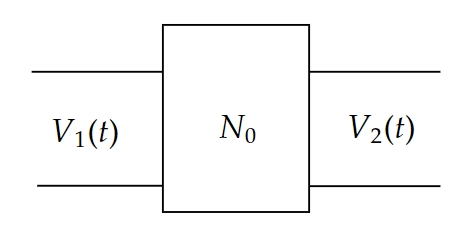
\includegraphics[width=0.3\textwidth]{3.19.1.png}
	\caption{}
\end{wrapfigure}
电路用频域表示时,输入和输出信号的关系可用式 
\begin{equation}
  V_2(\omega) = V_1(\omega)H(\omega)
\end{equation}
其中 $\mathrm{H_1(t)}$ 称之为该系统的频率特性,它的幅值 $\mathrm{|H(\omega)|}$ 称为幅频特性。$\mathrm{|H(\omega)|}$ 只与系统的结构组成有关,而与输入信号无关。本次设计就是要研究简单的 $\mathrm{RL}$ 低通网络和 $\mathrm{RC}$ 高通网络的幅频特性。由上式得 $\mathrm{H(\omega) = \dfrac{V_2(\omega)}{V_1(\omega)}}$,两边取对数再乘以 $20$,则有 $\mathrm{20lgH(\omega) = 20lgV_2(\omega) - 20lgV_1(\omega)}$,
\begin{equation}
  N(\omega) = N_2(\omega) - N_1(\omega)
\end{equation}

\begin{figure}[htbp]
	\centering
	\subfloat[]{
		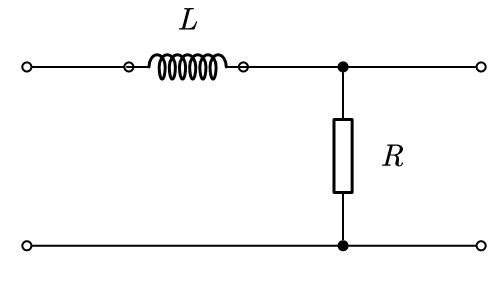
\includegraphics[width=0.3\textwidth]{3.19.2(a).png}
	}
	\subfloat[]{
		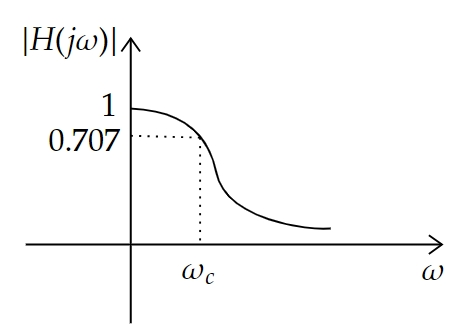
\includegraphics[width=0.3\textwidth]{3.19.2(b).png}
	}
	\caption{}
\end{figure}

根据电压电平的定义 $\mathrm{20lgV_2(\omega)}$ 和 $\mathrm{20lgV_1(\omega)}$ 正好分别与输出,输人电压电平的定义相符。故 $\mathrm{|H(\omega)|}$ 可由系统的输出信号 与输人信号的电平差 $\mathrm{N(\omega)}$ 求得。这是测量系统的频率特性的另一种方法。在实际工作中常常直接用 $\mathrm{N(\omega)}$ 來表征 $\mathrm{H(\omega)}$ 而不须求出 $\mathrm{H(\omega)}$,它清楚地表示了如图一线性时不变网络对任一个确定频率的正弦信号具有 $\mathrm{N(\omega)dB}$ 的衰减 [$\mathrm{N(\omega)}$ 为负值时]或增益[$\mathrm{N(\omega)}$ 为正值时]。
下图(a)是一个简单的低通网络,其频率特性:
\begin{equation}
  H(\omega) = \dfrac{V_2}{V_1} = \dfrac{1}{1 + j\dfrac{\omega L}{R}}
\end{equation}

经过推导变换,可得
\begin{equation}
  \left |H(\omega) \right | = \left |\dfrac{V_2}{V_1} \right | = \left |\dfrac{1}{1 + j\dfrac{\omega L}{R}}\right | = \left | \dfrac{1}{\sqrt{1 + (\dfrac{2\pi fL}{R})^2}} \right |
\end{equation}
$\mathrm{H(\omega) \sim \omega}$ 幅频特性曲线如下图(b)所示,在半功率频率 $f_c = \dfrac{1}{\tau} = \dfrac{R}{2\pi L}$ 时,$H(\omega) = 0.707$。

下图(a)是一个简单的高通网络,其频率特性为:
\begin{equation}
  H(\omega) = \dfrac{V_2}{V_1} = \dfrac{j\omega RC}{1 + j\omega RC}
\end{equation}

经过推导变换,可得
\begin{equation}
  \left |H(\omega) \right | = \left |\dfrac{V_2}{V_1} \right | = \left |\dfrac{j\omega RC}{1 + j\omega RC}\right | = \left | \dfrac{2\pi fRC}{\sqrt{1 + (2\pi fRC)^2}} \right |
\end{equation}
$\mathrm{H(\omega) \sim \omega}$ 幅频特性曲线如下图(b)所示,在半功率频率 $f_c = \dfrac{1}{\tau} = \dfrac{R}{2\pi L}$ 时,$H(\omega) = 0.707$。

\begin{figure}[htbp]
	\centering
	\subfloat[]{
		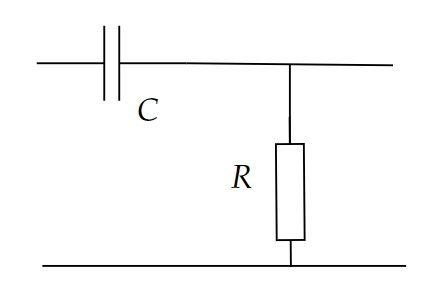
\includegraphics[width=0.3\textwidth]{3.19.3(a).png}
	}
	\subfloat[]{
		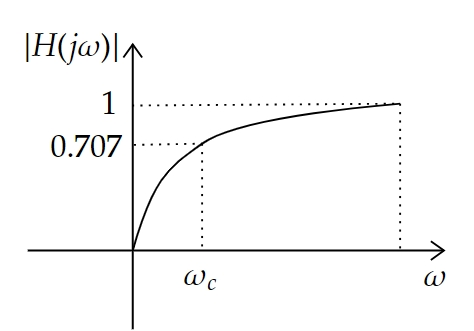
\includegraphics[width=0.3\textwidth]{3.19.3(b).png}
	}
	\caption{}
\end{figure}

\subsection*{五、说明}
本次实验是利用选频电平表分别测出线性网络的输人和输出电平,根据 $\mathrm{N(\omega)}$ 得到该网络的幅频特性。

信号源输出阻抗置 $50\Omega$。选频表输人阻抗置 $600\Omega$ 输人阻抗代替。

\begin{figure}[htbp]
	\centering
	\subfloat[]{
		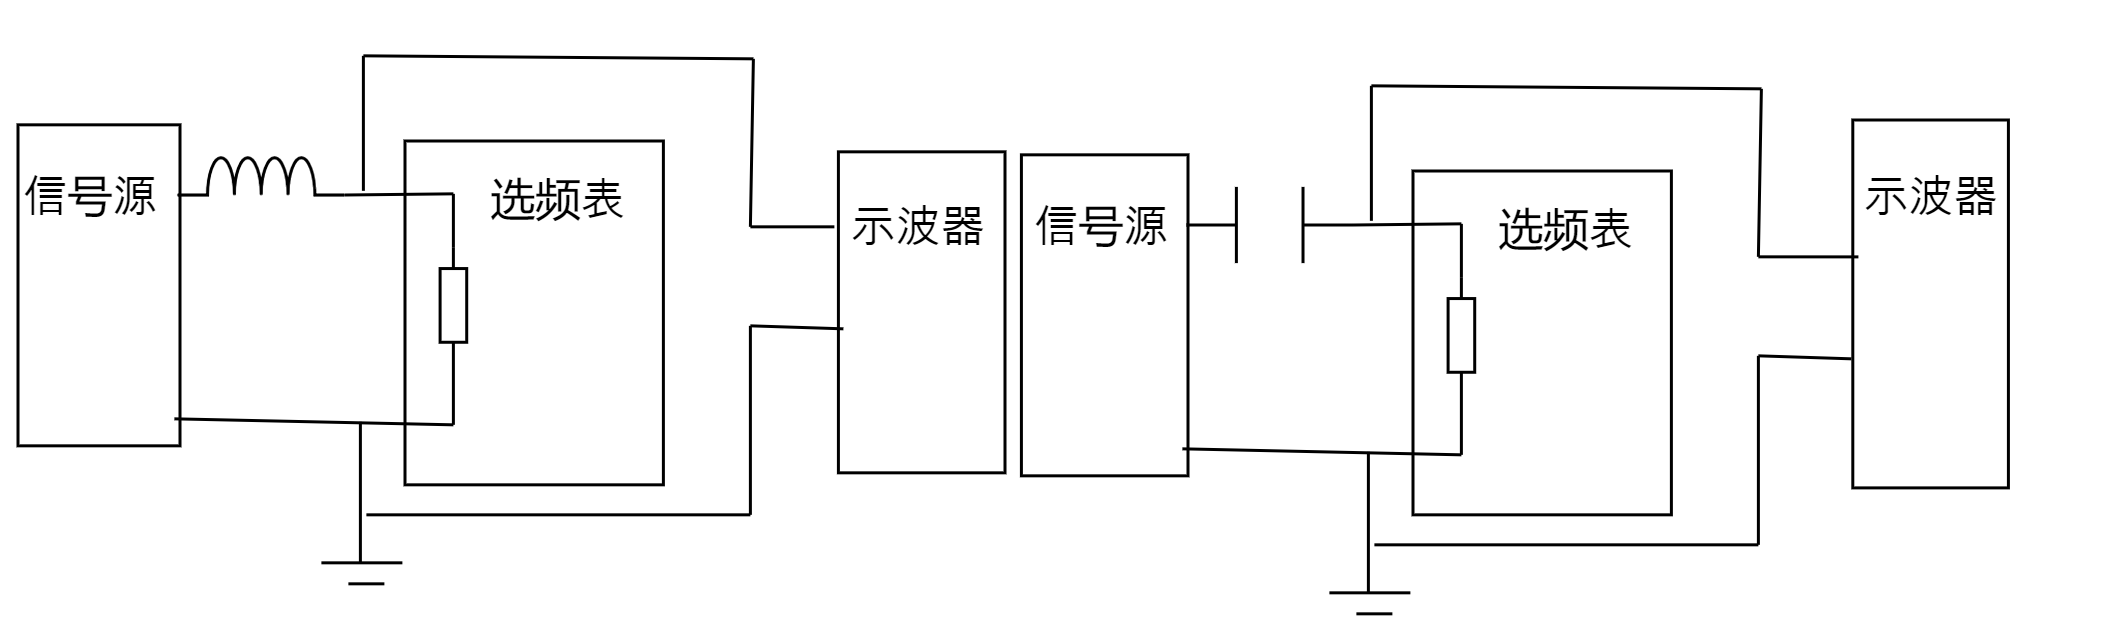
\includegraphics[width=0.7\textwidth]{3.19.4.png}
	}
	\caption{}
\end{figure}

\begin{enumerate}
	\item 测量输人信号频谱。
	\begin{enumerate}
    \item[A、] 电路图连接。(图 4)
    \item[B、] 用示波器和选频 表精确校准信号,输人信号为:周期 $7-200\mu s$,脉宽 $\tau =60 \mu s$:幅度 $V=5V$ 的矩形脉冲并画出波形图。
    \item[C、] 按表一第二栏的要求测出信号各次谱波的电平值 $N_1$。
    \item[D、] 观察示波器的波形并画在坐标纸上。
  \end{enumerate}
	\item 测量低通网络的输出电平。
	  \begin{enumerate}
      \item[A、] 电路如图 5 连接。
      \item[B、] 按表一第四栏的要求测出低通网络输出电平值 $\mathrm{N_d(\omega)}$。
      \item[C、] 观察示波器的波形并画在坐标纸上。
    \end{enumerate}
  \item 测量高通网络的输出电平。
    \begin{enumerate}
      \item[A、] 将图五电路中的电感 $L$ 改为 $0.01\mu F$ 的电容。
      \item[B、] 按表一第七栏的要求测出高通网络输出电平值 $N_d(\omega)$。
      \item[C、] 观察示波器的波形并画在坐标纸上.
    \end{enumerate}
  \item 分别计算高,低通滤波电路的幅频特性 $N_d(\omega)$。画出幅频特性曲线。
\end{enumerate}

\begin{figure}[htbp]
	\centering
	\subfloat[]{
		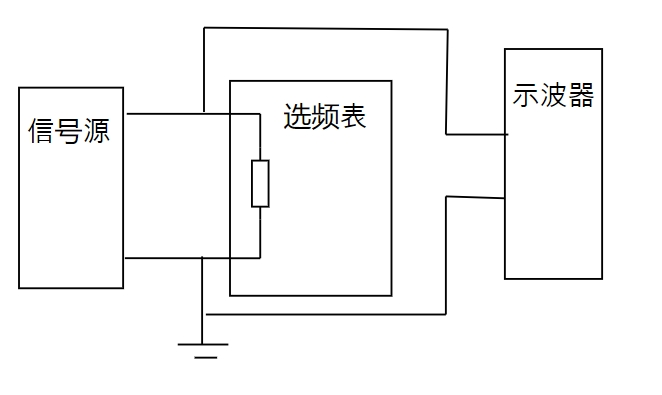
\includegraphics[width=0.6\textwidth]{3.19.5.png}
	}
	\caption{}
\end{figure}

\begin{table}[H]
  \renewcommand\arraystretch{1.7}
  \centering
  \caption{实际值测量}
  \begin{tabularx}{\textwidth}{|p{0.156\textwidth}|X|X|X|X|X|X|X|X|X|X|X|}
    \hline
    \multicolumn{2}{|c|}{$\mathrm{f(KH_z)}$} & 5 & 10 & 15 & 20 & 25 & 30 & 35 & 40 & 45 & 50 \\
    \hline
    输入信号电平 $N_1$ & 实测值 & 7.2 & 2.7 & -10.2 & -7.6 & -4.9 & -10.9 & -20.5 & -9.3 & -11.9 & -59.5 \\
    \hline
    \multirow{3}{*}{低通滤波电路 $N_d$} & 实测值 & &  &  &  &  & & &  & -22.7 & -30 \\
    \cline{2-12}
     & $N(\omega)$ & &  &  &  &  & & & & &  \\
     \cline{2-12}
     & $H(\omega)$ & &  &  &  &  & & & & &  \\
    \hline
    \multirow{3}{*}{低通滤波电路 $N_d$} & 实测值 & &  &  &  &  & & & & &  \\
    \cline{2-12}
    & $N(\omega)$ & &  &  &  &  & & & & &  \\
    \cline{2-12}
    & $H(\omega)$ & &  &  &  &  & & & & &  \\
    \hline
  \end{tabularx}
\end{table}
注:$H(\omega) = 10^{\frac{N(\omega)}{20}}$

\begin{table}[H]
  \renewcommand\arraystretch{1.7}
  \centering
  \caption{理论值计算}
  \begin{tabularx}{\textwidth}{|p{0.156\textwidth}|X|X|X|X|X|X|X|X|X|X|X|X|}
    \hline
    \multicolumn{2}{|c|}{$\mathrm{f(KH_z)}$} & 5 & 10 & 15 & 20 & 25 & 30 & 35 & 40 & 45 & 50 \\
    \hline
    \multirow{3}{*}{RL电路} & $N(f)$ & -0.52 & -1.78 & -3.31 & -4.81 & -6.20 & -7.45 & -8.58 & -9.60 & -10.52 & -11.36
    \\
    \cline{2-12}
     &$H(f)$ & 0.94 & 0.81 &	0.68 & 0.57	& 0.49 & 0.42 &	0.37 & 0.33 & 0.30 & 0.27
    \\
    \hline
    \multirow{3}{*}{RC电路} & $N(f)$ & -14.65 & -9.05 &	-6.16 & -4.41 &	-3.28 &	-2.51 & -1.97 & -1.58 &	-1.30 & -1.08
    \\
    \cline{2-12}
     & $H(f)$ & 0.19 & 0.35	& 0.49 & 0.60 &	0.69 & 0.75 &	0.80 & 0.83 &	0.86 & 0.88
    \\
    \hline
  \end{tabularx}
\end{table}

\end{document}
